\documentclass{beamer}
\renewcommand\thesection{\arabic{section}}
\newcommand{\myfont}{\rmfamily\normalsize\upshape\mdseries}
\newcommand{\degree}{^\circ}
\title{\sffamily Exercises for Mid 1}
\institute[UM-SJTU JI]{University of Michigan-Shanghai Jiao Tong University Joint Institute}
\author{Kulu}
\usepackage{graphicx}
\usepackage{picinpar}
\usepackage{indentfirst}
\usepackage{chemformula}
\usepackage{geometry}
\usepackage{subfigure}
\usepackage{appendix}
\usepackage{amsfonts,amsmath,amssymb}
\usepackage{enumerate}
\usepackage{float}
\usepackage{geometry}
\usepackage{latexsym}
\usepackage{listings}
\usepackage{multicol,multirow,multido}
\usepackage{tabularx}
\usepackage{ulem}
\usepackage{tikz}
\usepackage{xcolor}
\usepackage{cite}
\usepackage{setspace}
\usepackage{hyperref}
\usepackage{textpos}
\usepackage{booktabs}

\usetheme[dove]{Boadilla}
\usecolortheme{dolphin}
\useoutertheme{miniframes}
\begin{document}
\usebackgroundtemplate{\tikz\node[opacity=0.07]{
        \centerline{
\includegraphics[
                height=\paperheight]{kulu.jpg}}
    };}
\begin{titlepage}
    \begin{center}
        VV186 - Honors Mathmatics II
    \end{center}
\end{titlepage}
\myfont

\section{Sets}
\begin{frame}
    \frametitle{Exercise: Points}
    Please identify the interior, exterior, boundary and accumalation
    points of the set
    $$\{\frac{1}{z}:z\in \mathbb{Z}\backslash\{0\}\}\cup (\bigcap_{j=1}^\infty(-2-\frac{1}{j},-1+\frac{1}{j}))$$
\end{frame}

\begin{frame}
    \frametitle{Exercise: Bounds}
    \begin{figure}[htbp]
        \centering
        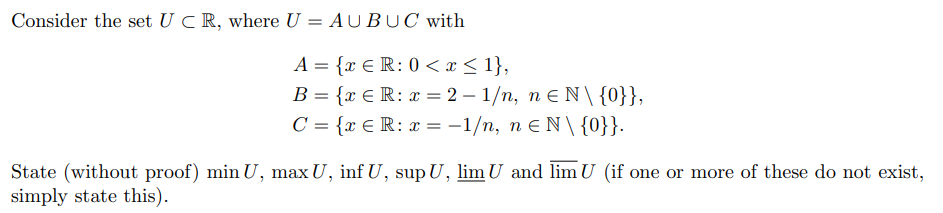
\includegraphics[width=12cm]{boundExercise.png}
    \end{figure}
\end{frame}

\section{Sequence}
\begin{frame}
    \frametitle{Exercise: Limit and Accumulation Point}
    \textcolor{red}{Easy, but check whether you should only USE WORDS !}
    \begin{figure}[htbp]
        \centering
        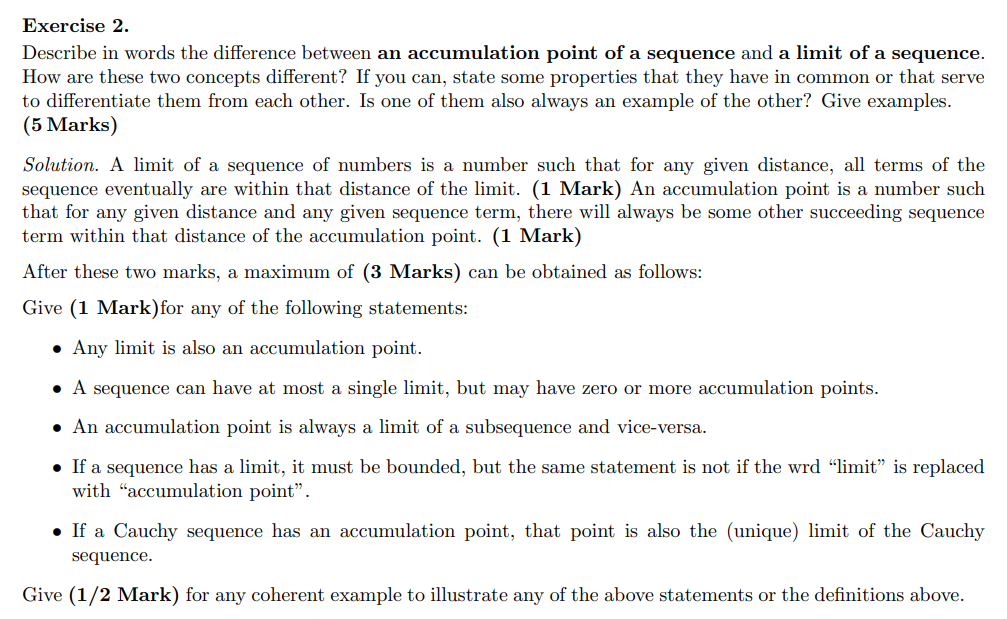
\includegraphics[width=10cm]{concept.png}
    \end{figure}
\end{frame}


\begin{frame}
    \frametitle{Exercises: Find limits for a recursively defined sequence}

    Just briefly discuss the methods. \textcolor{red}{Check details by yourself later.}
    \begin{figure}[htbp]
        \centering
        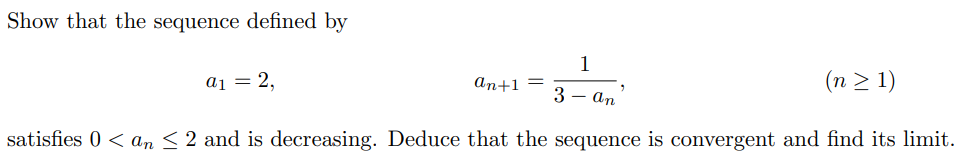
\includegraphics[width=12cm]{sequenceExercise.png}
    \end{figure}
\end{frame}


\begin{frame}
    \begin{figure}[htbp]
        \centering
        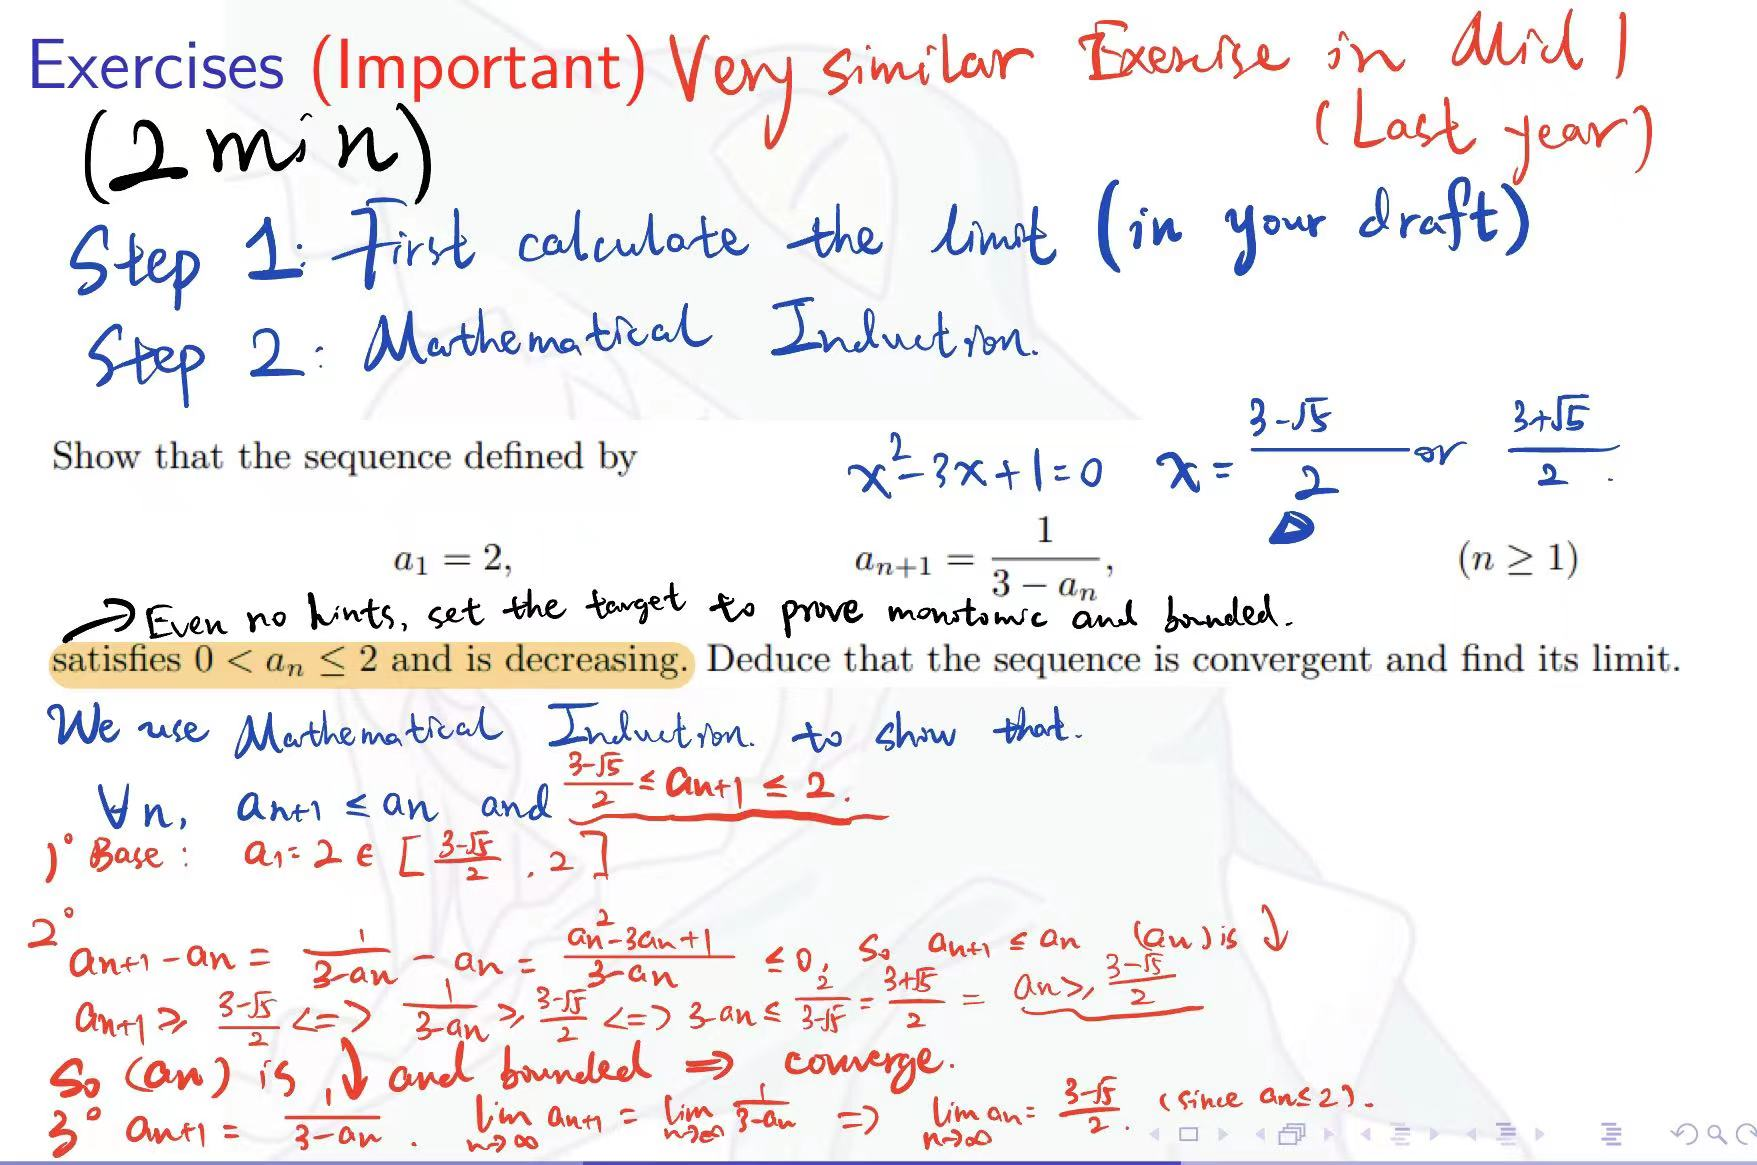
\includegraphics[width=12cm]{answerLimit.png}
    \end{figure}
\end{frame}


\begin{frame}
    \frametitle{Exercise: Upper Limits and Lower Limits}
    First recall their definitions, their properties...
    \begin{figure}[htbp]
        \centering
        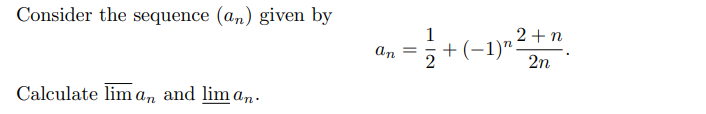
\includegraphics[width=10cm]{calculate.png}
    \end{figure}
\end{frame}


\begin{frame}
    \frametitle{Exercise: Upper Limits and Lower Limits}

    Given $(x_{n})$ a real bounded sequence, prove that:

    \vspace*{1em}
    \quad (1) $\forall \epsilon>0, \exists N\in \mathbb{N}$, $\forall n>N$, $x_{n}$<$\overline{lim}(x_{n})+\epsilon$.

    \vspace*{1em}
    \quad (2) $\forall \epsilon>0, \forall k$, $\exists n_{k}>k$, $x_{n_{k}}>\overline{lim}(x_{n})-\epsilon$.
\end{frame}

\begin{frame}
    \frametitle{Exercise: Upper Limits and Lower Limits}
    A valuable question asked in piazza.

    For a real bounded sequence $(a_{n})$, prove that if ran$(a_{n}$) doesn't have a maximum, then sup ran($a_{n}$) = $\overline{lim} a_{n}$.

    \vspace{5em}
    First recall the definition of ran$(a_{n})$. Divide the procedure of the exercise into several steps, set up your goal!
\end{frame}

\begin{frame}
    \frametitle{Exercise: Upper Limits and Lower Limits}
    Let $(a_{n})$ and $(b_{n})$ be two bounded real sequences. Prove that:
    \begin{equation*}
        \underline{lim}a_{n}+\underline{lim}b_{n} \leq \underline{lim}(a_{n}+b_{n}) \leq \overline{lim}a_{n}+\underline{lim}b_{n} \leq \overline{lim}a_{n} +\overline{lim}b_{n}.
    \end{equation*}
\end{frame}

\begin{frame}
    \frametitle{Exercise: Metric Space}
    Just briefly discuss the methods. \textcolor{red}{Check details by yourself later.}

    A metric space is complete when all cauchy sequence in this metric space converges.
    \begin{figure}[htbp]
        \centering
        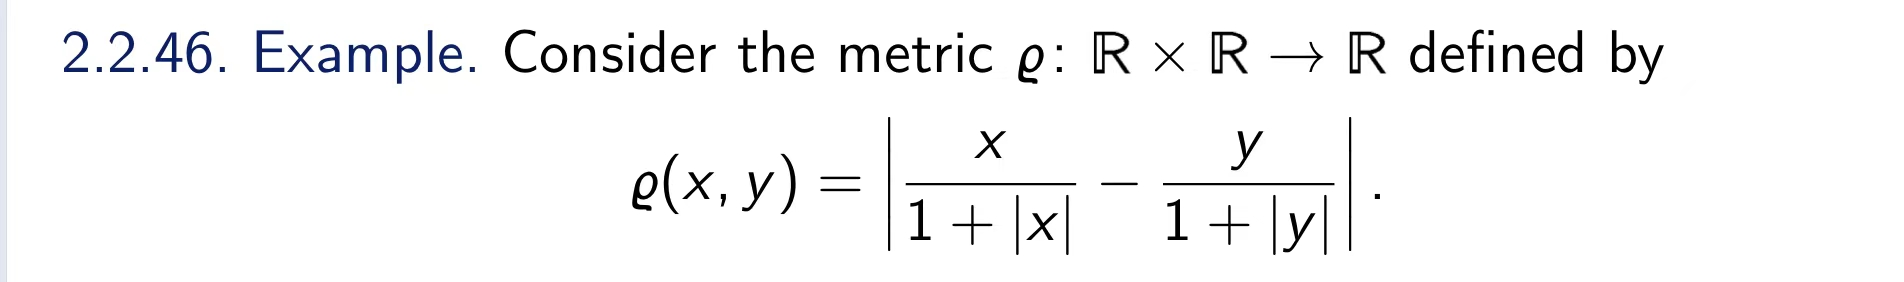
\includegraphics[width=12cm]{complete.png}
    \end{figure}
    Prove that the metric space $(\mathbb{R},\rho)$ is incomplete by analyzing the sequence: $a_{n}=n$.
\end{frame}

\begin{frame}
    \begin{figure}[htbp]
        \centering
        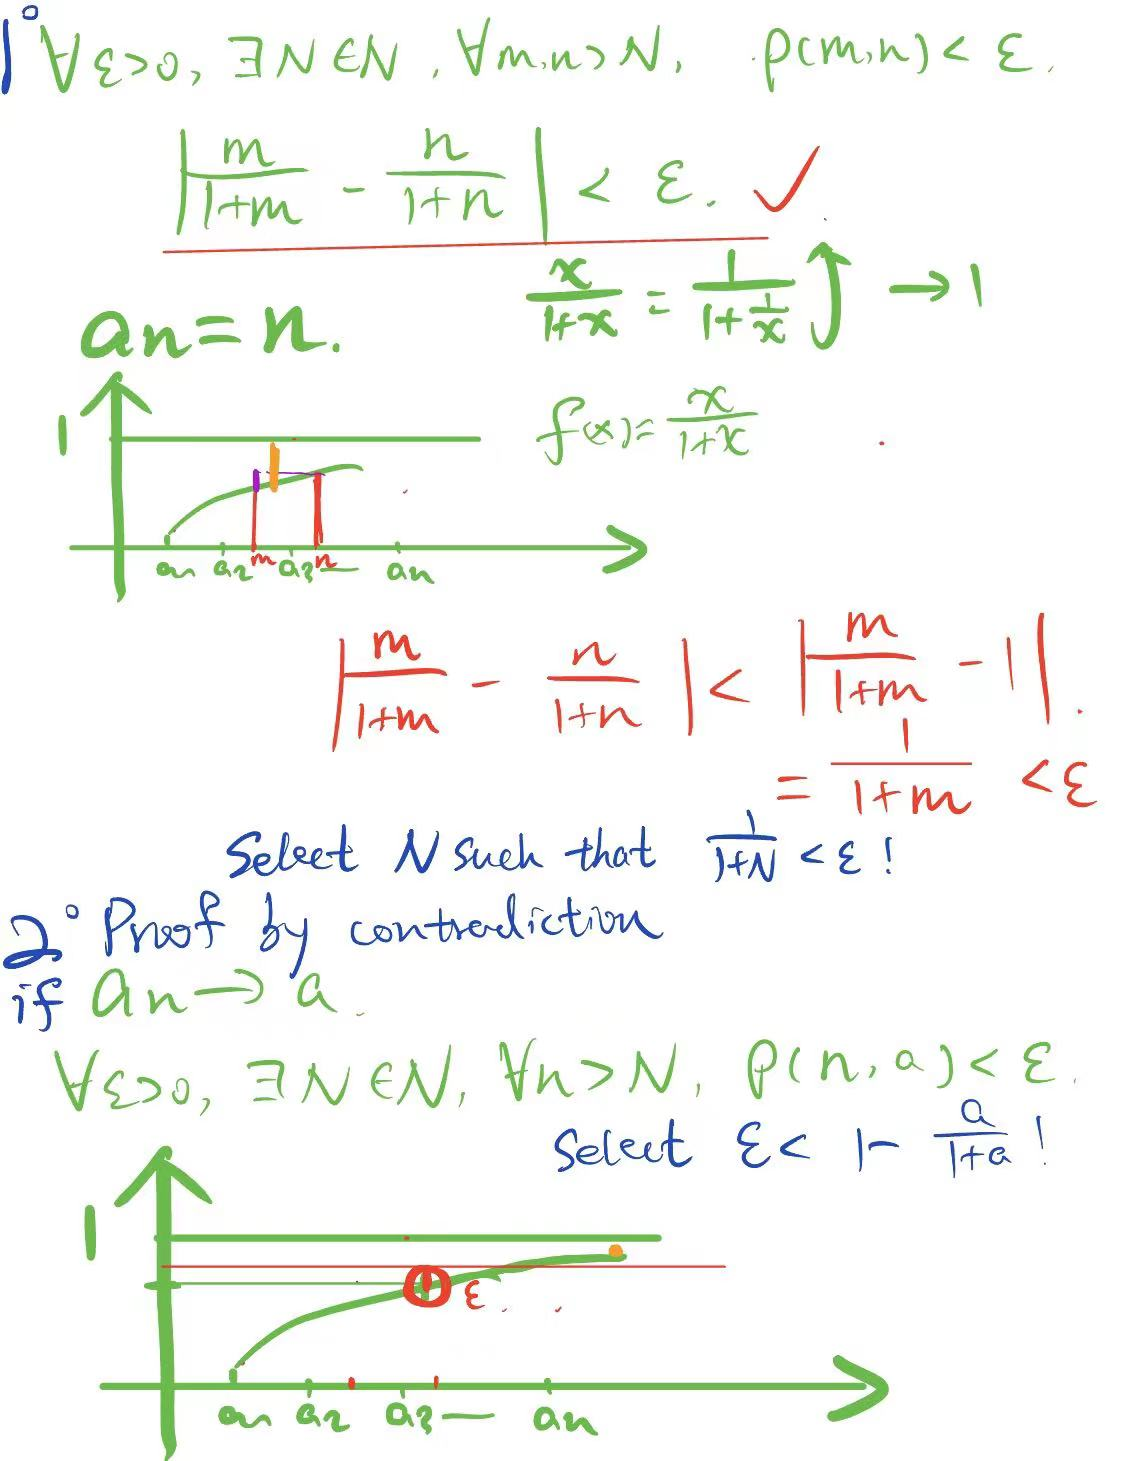
\includegraphics[width=6cm]{answerMetric.png}
    \end{figure}
\end{frame}

\begin{frame}
    \frametitle{Exercise \textcolor{red}{Important!} (A Former Midterm Question)}
    TAs have discussed this exercise in their RC3.

    Just briefly discuss the methods. \textcolor{red}{Check details by yourself later.}

    \vspace{2em}
    Prove that every Cauchy sequence has at most one accumulation point.

    \vspace{2em}
    Tips:
    \begin{itemize}
        \item You should work on an abstract metric space, using $\rho $ instead of $| \cdot |$.
        \item \textcolor{red}{Visualize to help you think !}
    \end{itemize}
\end{frame}

\begin{frame}
    \begin{figure}[htbp]
        \centering
        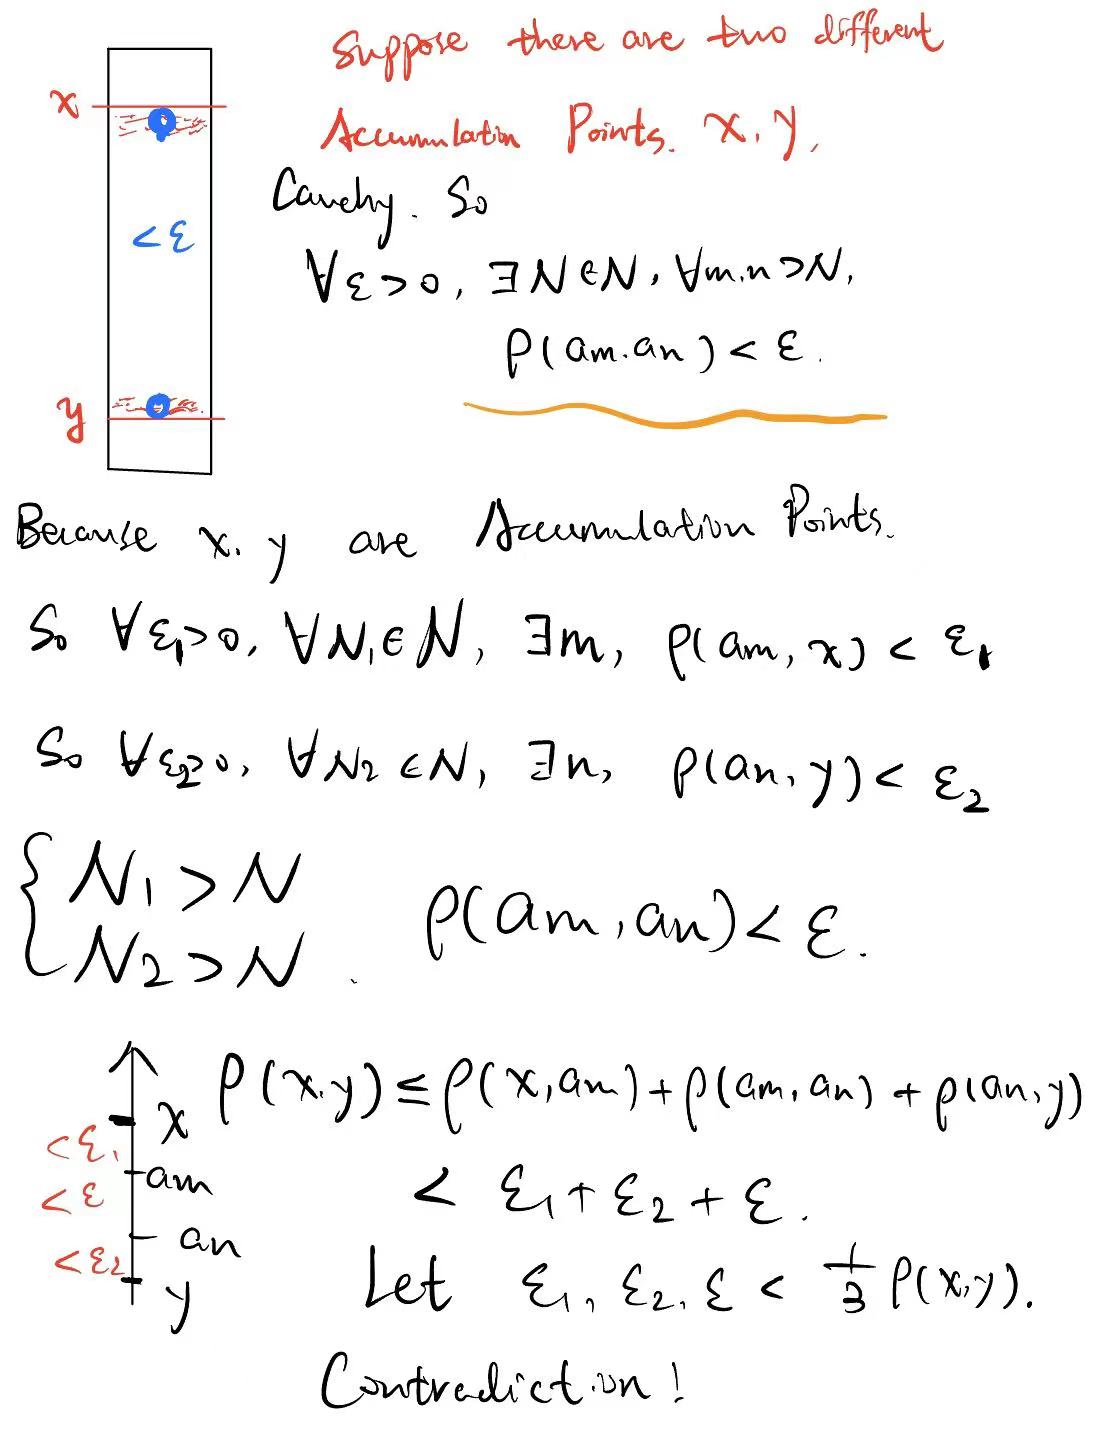
\includegraphics[width=6cm]{answerMetric2.png}
    \end{figure}
\end{frame}

\section{Function}
\begin{frame}
    \frametitle{Exercise: Big O and Small o}
    First recall the definition...
    \begin{figure}[htbp]
        \centering
        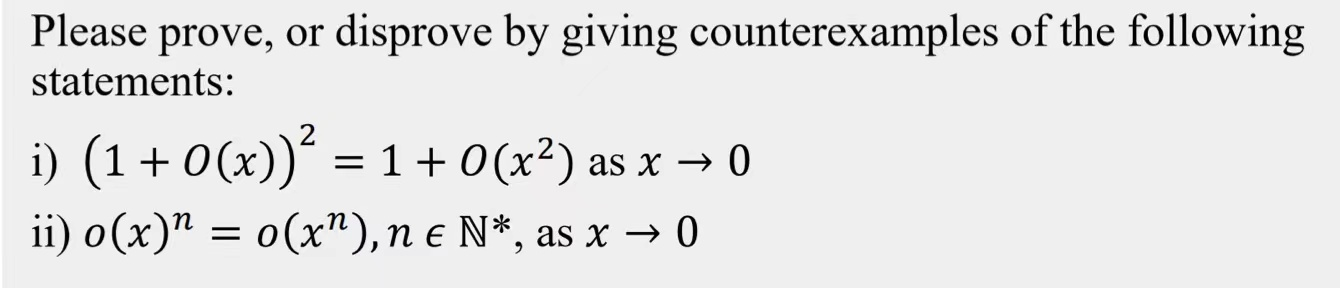
\includegraphics[width=12cm]{bigOsmallo.png}
    \end{figure}
\end{frame}


\begin{frame}
    \frametitle{Exercise: Small o and limits}
    A function f(x) satisfies that: $\underset{x\rightarrow 0}{lim}f(x)$=0. And f(x)-f($\frac{x}{2}$)=o(x) (x$\rightarrow$0). Prove that:

    \begin{center}
        f(x) = o(x) (x$\rightarrow$ 0)
    \end{center}

\end{frame}

\begin{frame}
    \frametitle{Exercise: Continuous and Uniformly Continuous}
    A function f(x) is continuous on [a,+$\infty$), and $\underset{x\rightarrow \infty}{lim}f(x)$ exists. Prove that:

    \begin{center}
        f(x) is uniformly continuous on [a,+$\infty$)
    \end{center}
\end{frame}

\begin{frame}
    \frametitle{Exercise: Continuous and Uniformly Continuous}
    It has been proved in lecture that: if f and g are two functions continuous at x. Then f+g and f $\cdot$ g are also continous at x.

    \vspace{1em}
    What about uniformly continous properties ?

    f(x) and g(x) are two uniformly continuous real functions defined in [0,+$\infty$).

    (1) Prove that:
    Function h(x) = f(x) + g(x), h(x) is also uniformly continuous.

    (2) Given that g(x) is bounded. Function h(x) = f(x)g(x). Is h(x) also uniformly continuous ?


\end{frame}

\begin{frame}
    \frametitle{Exercise: Continuous and Uniformly Continuous}
    \begin{figure}[htbp]
        \centering
        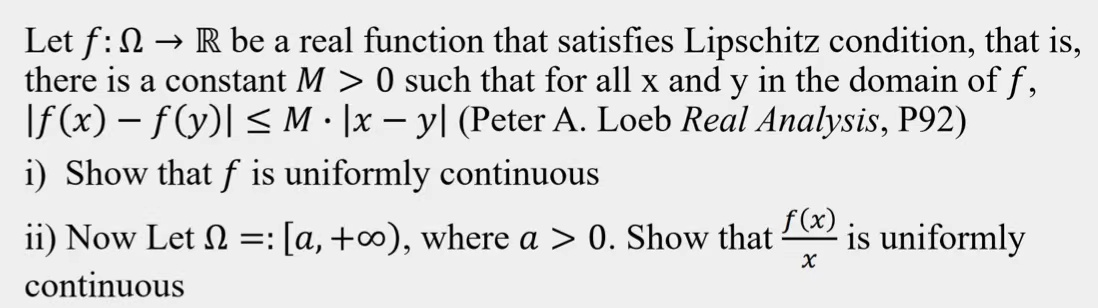
\includegraphics[width=12cm]{exerciseContinuous.png}
    \end{figure}
\end{frame}


\begin{frame}
    \frametitle{Exercise: Continuous and Uniformly Continuous}
    Function f(x) is defined on ($-\infty,+\infty$). Satisfying that $\forall x,y \in \mathbb{R}$,
    \begin{equation*}
        \left|f(x)-f(y)\right|\leq k\left|x-y\right|.
    \end{equation*}
    Here k is a constant satisfying that 0 < k < 1. Prove that:

    (1) $kx-f(x)$ is increasing.

    (2) $\exists c\in \mathbb{R}$, f(c)=c.

    (Hint: Bolzano Intermediate Value Theorem)
\end{frame}

\section{Reference}
\begin{frame}
    \frametitle{Reference}
    \begin{itemize}
        \item Vv186 Lecture Slides Professor Horst
        \item Vv186 Sample Exam from Professor Horst
        \item 2020 Vv186 TA-Huangqiyue
    \end{itemize}
\end{frame}

\section{At last}
\begin{frame}
    \frametitle{Say at the end of our RC}
    There are also many exercises in our regular RCs. And the most important and helpful exercises are all in your sample exam. Some of them are easy and many are hard. \textcolor{red}{If you can't tackle the exercises from today's RC and sample exam, that's totally normal !} Just try to understand the structure of the proof and get some thought from the solutions.

    Don't waste too much time on out-of-class materials. The most valuable materials will always be Professor's slide and homework. Get familiar with them !

    \vspace{1em}
    \begin{center}
        Hope you all relax and achieve good grade !
    \end{center}
\end{frame}


\end{document}